% *********************************************************************
% © 2021 Jeremy Sylvestre
%
% Permission is granted to copy, distribute and/or modify this document
% under the terms of the GNU Free Documentation License, Version 1.3 or
% any later version published by the Free Software Foundation; with no
% Invariant Sections, no Front-Cover Texts, and no Back-Cover Texts. A
% copy of the license is included in the appendix entitled “GNU Free
% Documentation License” that appears in the output document of this
% PreTeXt source code. All trademarks™ are the registered® marks of
% their respective owners.
%
% *********************************************************************

\newcommand*{\xmin}{0}
\newcommand*{\xmax}{2}
\newcommand*{\ymin}{0}
\newcommand*{\ymax}{10}

%
% DE is y' = r (M - y) (y - T) y
%
% We are using r = 1, T = 4, M = 8
%
% Solutions curves are
%   y = 4 [ 1 ± sqrt( A / (A - exp(-32t))) ]
% where
%   A = (y0 - 4)² / [ y0 * (y0 - 8) ]
% BUT
% have h.scaled solutions by factor of 10

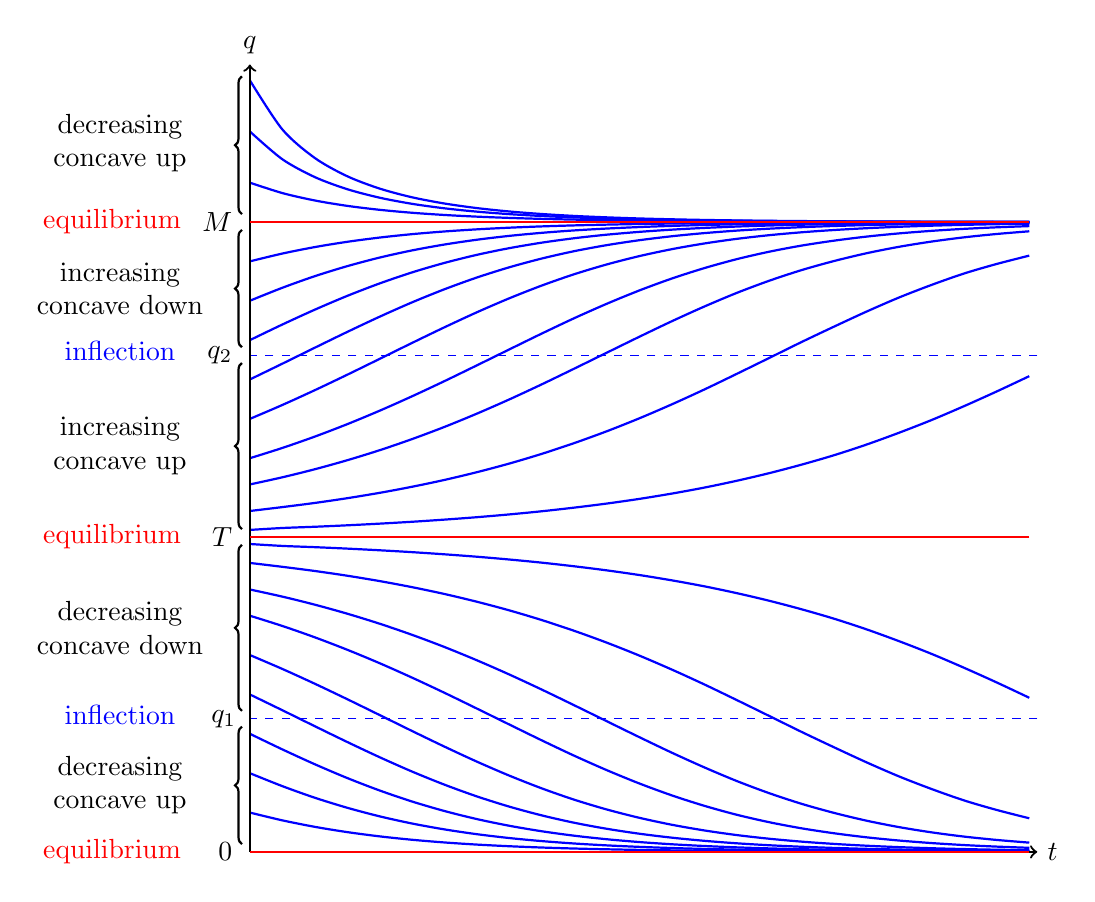
\begin{tikzpicture}
[
	closedpt/.style={circle,draw,fill,inner sep=0pt,minimum size=4pt},
	openpt/.style={circle,draw,inner sep=0pt,minimum size=4pt},
	xscale=5
]

	\draw[dashed,blue] (\xmax,1.691) -- (\xmin,1.691);
	\draw[dashed,blue] (\xmax,6.309) -- (\xmin,6.309);

	\node[left,xshift=-0.05cm] at (0,1.691) {$q_1$};
	\node[blue,yshift=0.05cm] at (-0.33,1.691) {inflection};

	\node[left,xshift=-0.1cm] at (0,6.309) {$q_2$};
	\node[blue,yshift=0.05cm] at (-0.33,6.309) {inflection};

	\draw[thick, decorate, decoration = {brace}, xshift=-0.02cm] (0,8.1) -- (0,9.85);
	\node[align=center] at (-0.33,9) {decreasing \\ concave up};

	\draw[thick, decorate, decoration = {brace}, xshift=-0.02cm] (0,6.409) -- (0,7.9);
	\node[align=center] at (-0.33,7.155) {increasing \\ concave down};

	\draw[thick, decorate, decoration = {brace}, xshift=-0.02cm] (0,4.1) -- (0,6.209);
	\node[align=center] at (-0.33,5.155) {increasing \\ concave up};

	\draw[thick, decorate, decoration = {brace}, xshift=-0.02cm] (0,1.791) -- (0,3.9);
	\node[align=center] at (-0.33,2.846) {decreasing \\ concave down};

	\draw[thick, decorate, decoration = {brace}, xshift=-0.02cm] (0,0.1) -- (0,1.591);
	\node[align=center] at (-0.33,0.845) {decreasing \\ concave up};

	% solutions with neg sqrt
	\foreach \q in {0.5,1,1.5,2,2.5,3,3.333,3.667,3.9} {
		\pgfmathparse{ (\q - 4) * (\q - 4) / (\q * \q - 8 * \q) }\edef\Acoeff{\pgfmathresult}%
		\draw[thick,blue,smooth,domain=0:1.98] plot (\x, { 4 * ( 1 - sqrt( \Acoeff / ( \Acoeff - exp(-32 * \x / 10) ) ) ) });
	}

	% solutions with pos sqrt
	\foreach \q in {4.1,4.333,4.667,5,5.5,6,6.5,7,7.5,8.5,9.15,9.8} {
		\pgfmathparse{ (\q - 4) * (\q - 4) / (\q * \q - 8 * \q) }\edef\Acoeff{\pgfmathresult}%
		\draw[thick,blue,smooth,domain=0:1.98] plot (\x, { 4 * ( 1 + sqrt( \Acoeff / ( \Acoeff - exp(-32 * \x / 10) ) ) ) });
	}

	% above q = T = 4, things become exponential
	% so invert to t = ...
	% so that we can control range instead of domain
	% \foreach \q in {4.07,4.18,4.3,4.5,4.72,5,5.25,5.5} {
	% 	\draw[thick,blue,smooth,domain=\q:\ymax] plot ({ (ln( \q * (4 - \x) / (\x * (4 - \q)) )) / 4 }, \x);
	% }

	% axes
	\draw[->,thick] (\xmin,0) -- (\xmax,0) node[right] {$t$};
	\draw[->,thick] (0,\ymin) -- (0,\ymax) node[above] {$q$};

	\foreach \q in {0,4,8} {
		\draw[red,thick] (1.98,\q) -- (\xmin,\q);
		\node[red] at (-0.35,\q) {equilibrium};
	}

	\node[left,xshift=-0.1cm] at (0,0) {$0$};
	\node[left,xshift=-0.1cm] at (0,4) {$T$};
	\node[left,xshift=-0.1cm] at (0,8) {$M$};

\end{tikzpicture}
